In this chapter, we introduce an inefficient consumer within a General Equilibrium scenario. As we have described in Chapter \ref{cha:GET}, standard Microeconomic Theory supposes that an agent faced with a choice of goods or services to purchase will maximize an expected utility function given his constraints \cite{mascolell}. It also predicts an equilibrium state resulting from these agents simultaneously and independently trying to optimize their own choices. 

Over the last decade these assumptions have been under
intense scrutiny \cite{bouchaud2008, KirmanBook}. Among other factors, the
2007-2008 mortgage crisis, for which the predictions made by
mainstream theories were ineffective in preventing, and the growing
empirical body of evidence being gathered in the field of Behavioral
Economics have shown that perfect rationality may be a very poor
proxy for the observed behavior of economic agents.

In fact, it has been shown that assuming zero
intelligence agents also produces realistic results \cite{Gode1993, Smith2003}
due to general statistical properties that may emerge in interacting
systems. As argued by the authors in \cite{Smith2003}, treating economic
agents as having full rationality and perfect knowledge is clearly a
significant assumption, so why not model the other end of the
spectrum?  It has been shown in \cite{Yakovenko00}
that, for an economy in which trades occur in a random fashion, the
wealth distribution at equilibrium is a Gibbs distribution. This is very close to
empirical observations for several countries, at least in the bulk of the distribution. By adding a rate of return on capital,
power law distributions are obtained \cite{Bouchaud2000}, what is again consistent with
empirical data for top earners.

As we have argued in Chapter \ref{cha:stat_mech}, Statistical Mechanics provides a robust framework, based on maximum entropy principles, for identifying and calculating macroscopic quantities relevant for the description of interacting  systems.
Within this framework, the temperature of a system represents how large observed
deviations from the ground state are likely to be. A zero temperature system is always at the configuration
which minimizes its energy function, while a system at infinite
temperature will be at any configuration allowed by its constraints with equal probability.

These considerations suggest a way to model consumers that may turn to be more realistic: the degree of rationality may be represented as a parameter within a Statistical Mechanics model with energy given by the negative utility. As we have discussed in Chapter \ref{cha:stat_mech}, a similar approach has already appeared in the contexts of Game Theory \cite{brock2001a, brock2001b, Blume93}
and General Equilibrium  \cite{Foley94, Foley96}. 

In this chapter, we present the equilibrium state for the Random Linear Economy model described in Chapter \ref{cha:RLE} at several different values of the temperature parameter $\beta$ and discuss the consequences of non zero temperature to some relevant macroeconomic quantities, namely, the consumer's average utility and the GDP. We will show that when we remove the $\beta \to \infty$ limit, the uniqueness in firm production at equilibrium vanishes and it's challenging to define prices. We offer an alternative method for arriving at finite temperature Gibbs distribution based on \cite{Marsili13} which preserves the price vector. Finally, we show that the utility behavior at positive temperatures is consistent with findings from Behavioral Economics, specifically, the fact that more options sometimes lead to worse decisions by costumers \cite{Lepper00, Schwartz02}.


On a technical note, although deviations from maximum utility are here named, in accordance with Economics literature, ``suboptimal'' or ``inefficient'', it is known in statistical inference and reinforcement learning that a ``softmax'' decision
rule can actually be beneficial in exploit-explore situations where the agent has incomplete knowledge about his available options and must, at each moment, decide whether to exploit known but possibly suboptimal actions or to explore risky but potentially more rewarding ones \cite{cohen2007}. In these situations, it is shown that the optimal strategy for choosing options is to adopt a "softmax" decision rule with a certain temperature parameter. Maybe the irrational consumer we describe in this chapter isn't so irrational after all.



\section{The Irrational Consumer}

We now turn to the question of how we can treat the consumer as an
agent that makes suboptimal choices while making as
little extra assumptions as possible for his behavior. We have argued in Chapter \ref{cha:stat_mech} that this type of question
is answered in Statistical Physics as the inference problem of finding the
probability distribution for $x$ that has maximum entropy given the
constraints that $P(x)$ must be a probability distribution and $U(x)$ must have a well defined average $\bar{U}$
\cite{Jaynes57}. The solution for this entropy maximization
problem is the Gibbs distribution:

\begin{equation}
  \label{eq:gibbs}
  P(x) = \frac{1}{Z(\beta)} e^{\beta U(x)},
\end{equation}

where $Z = \int_0^\infty dx \, e^{\beta U(x)}$ is the normalization term
and $\beta$ is the Lagrange multiplier that solves 

\begin{equation}
  \frac{1}{Z(\beta)} \int dx U(x) e^{\beta U(x)}  = \bar{U}
\end{equation}

As it is typical in Statistical Mechanics we can instead treat it as a parameter that controls how much we allow $\bar{U}(\beta)$ to deviate from its maximum value, found when $\beta \to \infty$. It's clear that in this limit the distribution collapses to a Dirac delta and the
inference reduces to the classical consumer problem. The parameter
$\beta$ provides a structured way to treat irrationality or uncertainty about the consumer decision. Moreover, we are certain that we are not making any additional assumptions about his behavior.

Because market clearing still holds, we can plug equation
\eqref{eq:market_clearing} directly into the Gibbs measure. The
probability of the consumer choosing a bundle $x$ is then transformed
to the probability of having the firms set a production vector $s$,
and is given by:

\begin{equation}
  \label{eq:inef_1}
  P(s | \xi, x_0) = \frac{1}{Z} e^{\beta U(x_0 + \sum_i s_i \xi_i)}\Theta(x_0 + \sum_i s_i \xi_i)
\end{equation}

Although this distribution is algebraically untractable except in the
$\beta \to \infty$ limit, we can find the expected values of
macroeconomic variables for the Random Linear Economy model by
sampling this distribution using a Metropolis-Hastings Monte Carlo
dynamic and averaging over the disorder $(\xi, x_0)$. We first find the average fraction of active
firms $\langle \phi \rangle_{\xi, x_0}$ at equilibrium as a
function of $\beta$. The results are shown in Figure
\ref{fig:s_pos_n}. We see that the inefficiency parameter $\beta$ has
changes the ``two regimes'' scenario of Figure \ref{fig:u_GDP_avg}, which is reproduced when $\beta > 10^5$. For lower values, the
monopolistic regime vanishes, and after a certain point the fraction of
active firms actually increases with $n$.

\begin{figure}[!ht]
  \centering
  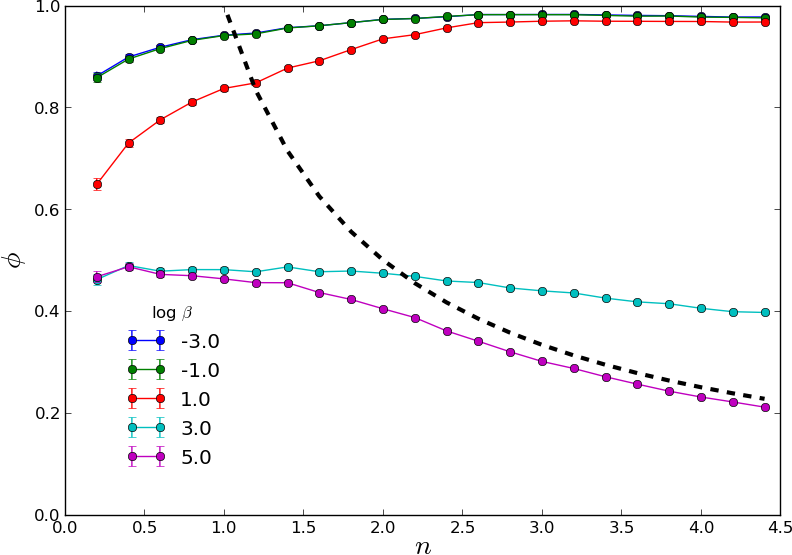
\includegraphics[width=.9\textwidth]{figs_inef/sPosMultipleBeta.png}
  \caption{Fraction of active firms $\phi$ as a function of the
    technological density $n$, for different values of $\beta$. The limit of active firms $\phi = 1/n$ is shown as the dashed line. When $\beta$ is high, around $10^5$, the fraction of active firms behaves as the original model shown in Chapter \ref{cha:RLE} and is always below the $1/n$ threshold. However, when $\beta$ decreases, the two regimes vanish and after a certain point the number of active firms increases with $n$. For all $\beta$ below a certain point, the limit $\phi < 1/n$ is violated and the economy no long supports a global price vector.}
  \label{fig:s_pos_n}
\end{figure}

More interesting, however, is the behavior of other macroeconomic
variables of the model. The utility at the $\beta \to \infty$ limit is always maximized by the consumer given his options, and therefore has to be an increasing function in $n$: a larger set of firms imply a wider set of choices, which the consumer can either take if it increases his utility or stay at his current bundle if it doesn't. When we allow for
suboptimal choice this is not always the case: the consumer can now change his final bundle due to "entropic" reasons, and it's not guaranteed that his expected utility will increase in this case. We compute the average utility per good
$\langle u \rangle$ for the consumer as a
function of $n$:

\begin{equation}
  \label{eq:inef_4}
  \langle u \rangle = \frac{1}{M} \langle U \rangle_{\xi, x_0} =
  \frac{1}{M} \int dx \int d\xi dx_0 U(x)
  \frac{1}{Z} e^{\beta U(x)} \Theta(x)
\end{equation}

As it can be seen in Figure \ref{fig:u_and_GDP}, for low temperatures
$\langle u \rangle$ behaves as expected. However, when we increase inefficiency, the average utility of the consumer starts
decreasing instead of increasing with the number of firms available
per good. This is quite interesting because it corroborates
empirical evidence from Behavioral Economics suggesting that choice can be excessive \cite{Lepper00, Schwartz02}: as the number of
options available to consumers increases, without perfect knowledge
and full rationally, the probability of them making mistakes also
increases.

We would like also to calculate the GDP of this economy, but we have
not defined the price vectors yet in this framework. For now we use the absolute amount of goods traded as a
proxy for economic activity, i.e., the economic activity $\Lambda$ is
given by

\begin{equation}
  \label{eq:inef_6}
  \Lambda = \frac{1}{M} \sum_{\mu = 1}^M \left| x_\mu - x_0^\mu \right|
\end{equation}

We see in the simulation results on the right panel of Figure \ref{fig:u_and_GDP} that
the economic activity always increases as as function of the
technological density $n$, but the rate of increase in $\Lambda$ also
increases with the inefficiency, as opposed to the utility. This is a
very peculiar behavior: suboptimal choice makes the amount of goods
traded in the economy increase as a whole, but the consumer's utility falls
because more exchanges are made inefficiently.

\begin{figure}[!ht]
  \centering
  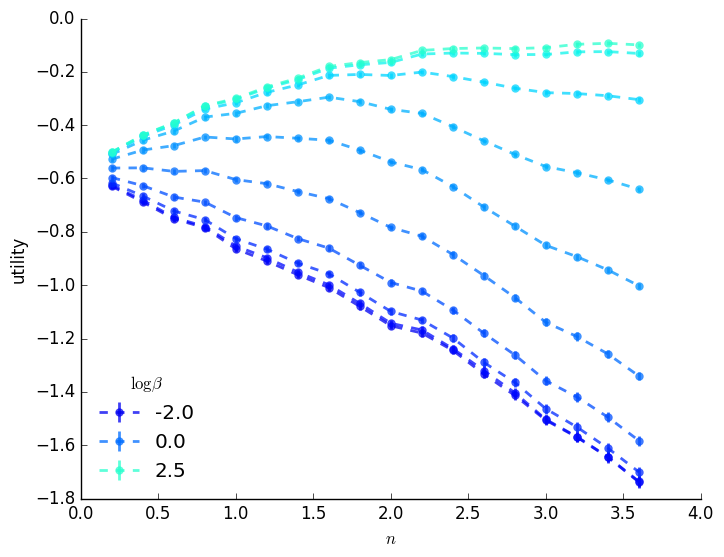
\includegraphics[width=.45\textwidth]{figs_inef/utility.png}
  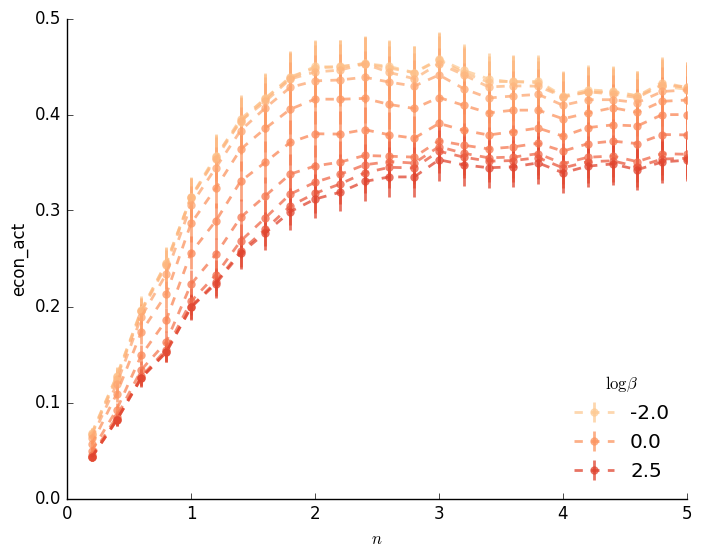
\includegraphics[width=.45\textwidth]{figs_inef/econ_act.png}
  \caption{\textbf{(Left)} Average consumer's utility per good as a function of the technological density $n$, for
    different values of $\beta$. For high values of $\beta$, an increase in the number of options available always increases the consumer's utility, just like the rational case presented on Chapter \ref{cha:RLE}. However, after a certain degree of inefficiency the utility decreases as one increases the number of choices. \textbf{(Right)} Average economic activity per good for the
    economy as a function of $n$. Unlike the utility, the economic activity always increases with the number of choices, increasing even further when the consumer is inefficient.}
  \label{fig:u_and_GDP}
\end{figure}

These results, however, have not come without drawbacks. Whereas originally
the prices were uniquely defined by the first order condition of the
consumer's optimization problem, in this new framework there is no
such restraint: given a probability distribution $P(x | \xi, x_0)$
finding the resulting price vector is an ill defined problem. In
fact, any vector $p$ that satisfies

\begin{equation}
  \label{eq:inef_3}
p \cdot \xi_i = 0, \text{ for all } i \text{ if } s_i > 0  
\end{equation}
is a candidate for global price. However, we have $N_a$ equations
of this type, one for each active firm, and $M$ unknown variables
$p_\mu$. It's straightforward to conclude that there is a threshold $N_a = M$ for
which the above system of equations has a solution. If we assume that all firm
technologies $\xi_i$ are linearly independent, then for any $N_a$
above $M$, there's no price vector $p$ that simultaneously satisfies
the zero profit constraint for all firms. In terms of $\phi$, this
means that for $\phi > 1/n$ there is no global price vector $p$ that
supports the economic activity observed. The curve $\phi = 1/n$ is plotted as
the dashed black curve in Figure \ref{fig:s_pos_n} and we see that
only when the consumer is very close to perfect rationality the market stays in this
region for all values of $n$. For higher inefficiency, there is always
a threshold where no global prices exist. This does not mean that there are no
market transactions taking place, only that prices must be
defined locally, and we have no way of defining this more precisely
without additional assumptions.

\section{Unobserved Utility}

We can solve this indefinition of prices by altering the setup so that
the equilibrium is still obtained from a maximization problem of the
consumer. In \cite{Marsili13} Marsili et al show that a complex system that maximizes an objective function $U(\vec{s})$ that can be decomposed as

\begin{equation}
    U(s) = u(s_v) + v(s_h | s_v),
\end{equation}

where $u(s_v)$ is the known component and $v(s_h | s_v)$ is the hidden component which we assume is unobservable. If $v(s_h | s_v)$ is not heavy tailed, then the observed part $s_v$ is Gibbs distributed:

\begin{equation}
  P(s_v) = \frac{1}{Z}e^{\beta u(s_v)},
\end{equation}

where $\beta$ is a function of the number of known and unknown variables.

We can use this framework to arrive at the Gibbs distribution in the Random Economies through a stochastic perturbation in the
consumer's utility function that we will treat as unobserved. We call
$U_t$ the ``true'' utility function and write it as

\begin{equation}
  \label{eq:inef_2}
  U_t(x) = U(x) + h \cdot x,
\end{equation}
where $h$ is a $M$ dimensional vector where all entries are independent
exponential random variables with scale $\lambda$. This term
represents unknown quantities about the consumer's utility which we do
not have access to, such as shocks in preference which change
daily. We point out that the true utility function $U_t$ is still a
concave function and therefore the equilibrium is still unique and
well behaved.

As shown in \cite{Marsili13}, the resulting probability
distribution for $x$ when the consumer is maximizing the utility
distribution $U_t(x)$ is a Gibbs distribution for $U(x)$. This
allows us to treat it as a framework where the consumer does not
choose the ``optimal'' for the utility $U(x)$, but we still have a
well defined price vector which is the result of the first order
conditions from the maximization problem. For the utility
$U(x) = \sum_\mu \log(x_\mu)$ the price of a good is given by
$p_\mu = \partial_\mu U_t(x) = \frac{1}{x_\mu} + h_\mu$.

The results for the fraction of active firms $\phi$ are the same as the results obtained in Chapter \ref{cha:RLE}, because it still remains a maximization problem
with the same constraints and with a concave utility function, equivalent to a convex energy function which has a single, replica
symmetric solution for the ground state. Therefore, we still have a
competitive regime for $n<2$ where around half of the firms are
active, which collapses to a monopolistic regime when $n>2$ where few
firms are active and $\phi$ reaches zero asymptotically.

However, the behavior of the macroeconomic quantities described above,
average utility per good $\langle u \rangle$ and GDP $Y$, which we
are now able to calculate using the good prices, are similar to the
inefficient consumer framework described above as can be seen on
figure \ref{fig:u_and_GDP_stoc}, where we plot the results of the
maximization process for the true utility for several values of the
scale $\lambda$ for the exponential distribution of $h_\mu$.

\begin{figure}[!ht]
  \centering
  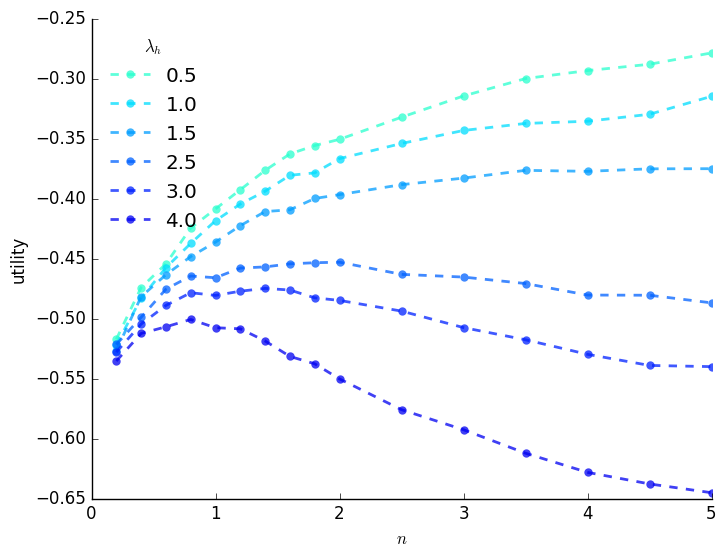
\includegraphics[width=.45\textwidth]{figs_inef/stoc_utility.png}
  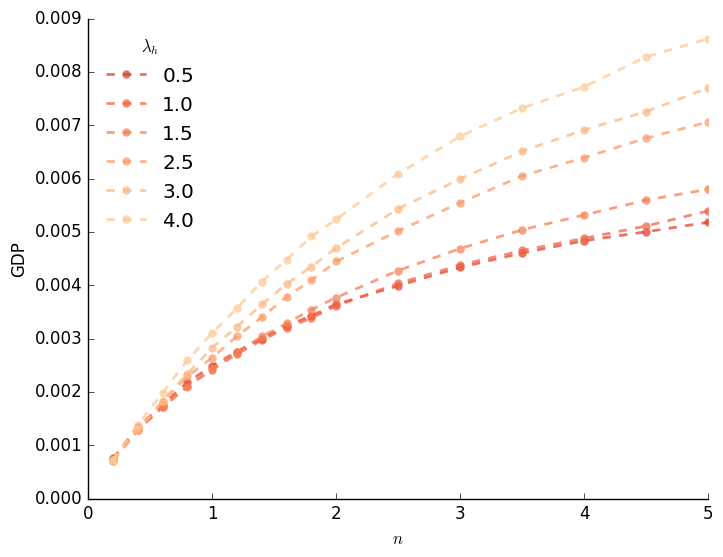
\includegraphics[width=.45\textwidth]{figs_inef/stoc_GDP.png}
  \caption{\textbf{(Left)} Average consumer's observed utility per good as a
    function of the technological density $n$ in the unobserved utility framework, for
    different values of $\beta$. Just like in the first scenario, the utility behaves as expected for very small perturbations, but large perturbations make it decrease with the number of choices available. \textbf{(Right)} Average GDP for the
    economy as a function of $n$. Again in this case, just like the original scenario, GDP rises even further when the consumer is inefficient and has a lower utility.}
  \label{fig:u_and_GDP_stoc}
\end{figure}

As in the previous case, after a certain value of $\lambda$ the
observed utility starts decreasing with $n$, while the GDP has an
increased rate of growth with $n$ for larger lambdas.

The downside of this approach, of course, is that we had to introduce
some extra assumptions about the consumer's utility. However,
as it is pointed out in \cite{Marsili13}, the Gibbs shape for
the known part of the function is dependent only on very general
conditions for the unknown part, and therefore the results we have
obtained are qualitatively robust to different choices in the
perturbed utility.

\section{Conclusion}

In this chapter we have shown two simple ways of treating
inefficient or irrational consumer behavior in a general equilibrium
setting, via the Random Linear Economies model presented above. Both
cases, however, are applicable to any General Equilibrium setting. We
have shown that when the consumer does not choose the bundle that
strictly maximizes his utility, the behavior of macroeconomic
quantities such as average utility and GDP have diverging slopes as a
function of the number of options available on his consumption set.

Crucially, as inefficiency in choice increases the consumer finds
itself being overwhelmed with the number of choices possible and
chooses poorly. This corroborates some well known results in
behavioral economics \cite{Lepper00, Schwartz02} and it's very
encouraging that we can reproduce these empirical behaviors in this
simple setup.

We also observe that GDP growth increases, as opposed to the utility,
with the increase in choice inefficiency. A higher number of options
may result in poorer choices, but it also leads to increased economic
activity. From a country perspective, therefore, it's desirable that
its consumers are not completely rational agents. Less efficiency in
choice leads to an increase in GDP and therefore in tax revenues. If
one thinks of country development as an evolutionary process, there is
would be selective pressure for higher inefficiency, and countries
with perfectly rational consumers would disappear due to lower
economic activity. However, if the average utility is a proxy for
individual fitness, then this would be similar to a ``emergence of
cooperation'' scenario usually dealt in Economics, where a rational
consumer would thrive in a country with low choice efficiency.

This is certainly too deep a conclusion to be arrived from just this
simple model. However, the results may be robust for other equilibrium
scenarios, and we hope this work sets the stage for future research
on this topic.